%% ****** Start of file template.aps ****** %
%%
%%
%%   This file is part of the APS files in the REVTeX 4 distribution.
%%   Version 4.0 of REVTeX, August 2001
%%
%%
%%   Copyright (c) 2001 The American Physical Society.
%%
%%   See the REVTeX 4 README file for restrictions and more information.
%%
%
% This is a template for producing manuscripts for use with REVTEX 4.0
% Copy this file to another name and then work on that file.
% That way, you always have this original template file to use.
%
% Group addresses by affiliation; use superscriptaddress for long
% author lists, or if there are many overlapping affiliations.
% For Phys. Rev. appearance, change preprint to twocolumn.
% Choose pra, prb, prc, prd, pre, prl, prstab, or rmp for journal
%  Add 'draft' option to mark overfull boxes with black boxes
%  Add 'showpacs' option to make PACS codes appear
%  Add 'showkeys' option to make keywords appear
\documentclass{revtex4}
%\documentclass[aps,prl,preprint,superscriptaddress]{revtex4}
%\documentclass[aps,prl,twocolumn,groupedaddress]{revtex4}
\usepackage[dvipdf]{graphicx}
%\usepackage{dcolumn}

% You should use BibTeX and apsrev.bst for references
% Choosing a journal automatically selects the correct APS
% BibTeX style file (bst file), so only uncomment the line
% below if necessary.
%\bibliographystyle{apsrev}

\begin{document}

% Use the \preprint command to place your local institutional report
% number in the upper righthand corner of the title page in preprint mode.
% Multiple \preprint commands are allowed.
% Use the 'preprintnumbers' class option to override journal defaults
% to display numbers if necessary
%\preprint{}

%Title of paper
\title{Determination of the Equilibrium Shape of a Freely Hanging Uniform Chain}

% repeat the \author .. \affiliation  etc. as needed
% \email, \thanks, \homepage, \altaffiliation all apply to the current
% author. Explanatory text should go in the []'s, actual e-mail
% address or url should go in the {}'s for \email and \homepage.
% Please use the appropriate macro foreach each type of information

% \affiliation command applies to all authors since the last
% \affiliation command. The \affiliation command should follow the
% other information
% \affiliation can be followed by \email, \homepage, \thanks as well.
\author{Physics 2501: Mechanics and Electromagnetism Laboratory}
%\homepage[]{Your web page}
%\thanks{}
%\altaffiliation{}
\affiliation{Dept. of Physics, University of Connecticut}
%\author{R.T. Jones}
%\affiliation{University of Connecticut}

%Collaboration name if desired (requires use of superscriptaddress
%option in \documentclass). \noaffiliation is required (may also be
%used with the \author command).
%\collaboration can be followed by \email, \homepage, \thanks as well.
%\collaboration{}
%\noaffiliation

\date{\today}

%\begin{abstract}
% insert abstract here
%\end{abstract}

% insert suggested PACS numbers in braces on next line
%\pacs{}
% insert suggested keywords - APS authors don't need to do this
%\keywords{}

%\setlength{\topmargin}{0in}

%\maketitle must follow title, authors, abstract, \pacs, and \keywords
\maketitle

% body of paper here - Use proper section commands
% References should be done using the \cite, \ref, and \label commands

%% The normal text is displayed in two-column format, but special
%% sections spanning both columns can be inserted within the page
%% format so that long equations can be displayed. Use
%% sparingly.
%%\begin{widetext}
%% put long equation here
%%\end{widetext}
%
%% figures should be put into the text as floats.
%% Use the graphics or graphicx packages (distributed with LaTeX2e)
%% and the \includegraphics macro defined in those packages.
%% See the LaTeX Graphics Companion by Michel Goosens, Sebastian Rahtz,
%% and Frank Mittelbach for instance.
%%
%% Here is an example of the general form of a figure:
%% Fill in the caption in the braces of the \caption{} command. Put the label
%% that you will use with \ref{} command in the braces of the \label{} command.
%% Use the figure* environment if the figure should span across the
%% entire page. There is no need to do explicit centering.
%
%%\begin{turnpage}
%% Surround figure environment with turnpage environment for landscape
%% figure
%% \begin{turnpage}
%% \begin{figure}
%% \includegraphics{}%
%% \caption{\label{}}
%% \end{figure}
%% \end{turnpage}
%
%% tables should appear as floats within the text
%%
%% Here is an example of the general form of a table:
%% Fill in the caption in the braces of the \caption{} command. Put the label
%% that you will use with \ref{} command in the braces of the \label{} command.
%% Insert the column specifiers (l, r, c, d, etc.) in the empty braces of the
%% \begin{tabular}{} command.
%% The ruledtabular enviroment adds doubled rules to table and sets a
%% reasonable default table settings.
%% Use the table* environment to get a full-width table in two-column
%% Add \usepackage{longtable} and the longtable (or longtable*}
%% environment for nicely formatted long tables. Or use the the [H]
%% placement option to break a long table (with less control than 
%% in longtable).
%
%
%% Surround table environment with turnpage environment for landscape
%% table
%% \begin{turnpage}
%% \begin{table}
%% \caption{\label{}}
%% \begin{ruledtabular}
%% \begin{tabular}{}
%% \end{tabular}
%% \end{ruledtabular}
%% \end{table}
%% \end{turnpage}
%
%% Specify following sections are appendices. Use \appendix* if there
%% only one appendix.
%%\appendix
%%\section{}
%

\section{Introduction}

Intuition suggests that a flexible chain with a uniform mass distribution
which is freely suspended under gravity from two fixed points will eventually
come to rest in a stable shape that is confined to the plane containing the
two suspension points and the center of the earth. Less obvious, however,
is the exact function that the contour of the chain traces out in that plane.
Casual observation suggests that the shape may be parabolic.  According to
Newtonian mechanics, the parabola does not satisfy the conditions for static
equilibrium in a uniform gravitational field.  As will be shown below, the
prediction from Newtonian statics is that only the shape described by the
hyperbolic cosine function is stable in uniform gravity.  Whatever its exact
mathematical form, the shape of a freely hanging uniform chain is called the
``catenary''.  In the period before the principles of geometry and
trigonometry were widely known, architects and masons knew that the shape
of a freely hanging chain, when it is turned upside-down, is the shape
required for building stable self-supporting arches such as those seen in
ancient castles, temples and cathedrals, stone bridges and aquaducts.
Without knowing much of what we call trigonometry today, these craftsmen
were able to determine this shape based on careful measurements of a hanging
chain, and reproduce it in inverted form in the arches they built. Because
of the important role this shape has played in human history, it has this
special name of catenary dedicated to it.

The catenary is not a single shape, but a family of shapes
which differ from each other in the ratio of the width to the height of the
arc, which describes the amount of dip that the chain undergoes between the
two points where it is suspended.  In this experiment you will measure two
particular members of the catenary family that you will chose, and test
whether their shapes are consistent with the parabola, the hyperbolic 
cosine, perhaps both, or even neither one.

The shape of the catenary is derived from Newton's Laws as follows. Consider
a uniform chain hanging freely under gravity from two fixed points at the
same height a distance $W$ apart, as shown in Fig.~\ref{catenaryfig}. A small
segment of the chain has been highlighted with a thick line in the figure for
emphasis, but it has the same mass per unit length λ as the rest of the chain
The free-body diagram in the figure shows that gravity acts downward on the
segment with force $gdm = g\lambda\sqrt{(dx)^2+(dy)^2}$.  The link
of the chain to the left pulls the segment of interest with tension $T_1$,
which is not the same as the tension $T_2$ being applied by the link to the
right. The static equilibrium condition requires that the vector sum of these
three forces be zero.

\begin{equation}
T_{2x} = T_{1x}
\label{eq:x-equil}
\end{equation}
\begin{equation}
T_{2y} = T_{1y} + g\lambda\sqrt{(dx)^2+(dy)^2}
\label{eq:y-equil}
\end{equation}

\begin{figure}
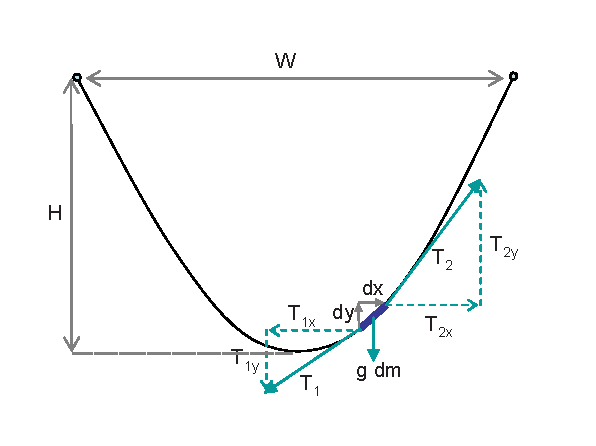
\includegraphics[width=4in]{catenaryfig.eps}
\caption{\label{catenaryfig}
Diagram of the experimental apparatus consisting of a uniform chain hanging
freely from two fixed points at the same height a distance $W$ apart. The
length $L$ of the chain is sufficiently larger than $W$ to allow it to hang
down a distance $H$ from the end points. The highlighted section indicates
a small segment of the chain of mass $dm$. A free-body diagram for the mass
$dm$ is superimposed. The symbols $T_1$ and $T_2$ represent the tension
forces from the remainder of the string that are acting on the two ends
of the small segment $dm$.}
\end{figure}

The condition that the chain is flexible means that the tension forces must
be tangent to the curve of the chain, that is
\begin{equation}
\frac{T_{1y}}{T_{1x}} = \frac{dy}{dx}
\label{eq:flex}
\end{equation}
Eq.~\ref{eq:x-equil} requires that the $x$-component of the tension force be
the same everywhere on the free-hanging portion of the chain, so the symbol
$T_0 = T_{1x} = T_{2x}$ will be used for to represent it. Eqs.\ref{eq:y-equil}
and \ref{eq:flex} combine to become
\begin{equation}
\frac{dT_y}{dx} = g\lambda\sqrt{1+\left(\frac{dy}{dx}\right)^2}
= \frac{d}{dx}\left(T_0 \frac{dy}{dx}\right)
\end{equation}
where Eq.~\ref{eq:flex} has been differentiated once to produce the
right-hand equation. This can be rewritten as
\begin{equation}
\frac{dy'}{dx} = \frac{g\lambda}{T_0}\sqrt{1+(y')^2}
\label{eq:diffeq}
\end{equation}
where y
where $y' = dy/dx$. This is a first-order non-linear ordinary differential
equation for $y'$.  The most general solution is
\begin{equation}
y' = \sinh{a(x-x_0)}
\label{eq:gensol}
\end{equation}
where the symbol $a$ has been introduced as shorthand for the constant
$g\lambda/T_0$. The function $\sinh$ is the hyperbolic sine function.
Its definition, together with its sister the hyperbolic cosine, are
\begin{eqnarray}
\sinh{x} &=& \frac{e^x - e^{-x}}{2} \nonumber \\
\cosh{x} &=& \frac{e^x + e^{-x}}{2} \nonumber
\end{eqnarray}
These hyperbolic functions obey trigonometric relations that are almost
the same as those for their companion functions the sine and cosine.
\begin{eqnarray}
\sinh{x} &=& \sqrt{\cosh^2{x}-1} \nonumber \\
\cosh{x} &=& \sqrt{\sinh^2{x}+1} \nonumber \\
\frac{d}{dx}\cosh{x} &=& \sinh{x} \nonumber \\
\frac{d}{dx}\sinh{x} &=& \cosh{x} \nonumber
\end{eqnarray}
These relations are needed to verify that Eq.~\ref{eq:gensol} is a solution
to Eq.~\ref{eq:diffeq}.  Undetermined integration constant $x_0$ must be
fixed by the boundary conditions. Integrating $y'$ one more time leads to
the solution for $y$,
\begin{equation}
y = y_0 + \frac{1}{a}\left(\cosh[a(x-x_0)] - 1\right)
\label{eq:solfory}
\end{equation}
where the constant of integration has been written such that $y_0$ is the
height of the chain at its minimum. Written in this form, $(x_0,y_0)$ is the
apex of the curve represented by the function $y(x)$. 

\section{Procedure}

A fine, flexible chain and large sheets of graph paper are needed for this
experiment. Measure the length of the chain and record its value as $L$,
together with its measurement error $\Delta L$. Using the chain as a plumb,
align the $y$-lines of the graph paper with the gravitational vertical as
precisely as possible and attach it to the cork board with tacks.
Suspend the chain from two pins so that the pins puncture the graph paper
at two points alone the same horizontal line. Make sure that there is enough
droop in the chain to make a precise measurement of the shape; somewhere
between 2:1 and 1:2 in the ratio $W:H$ would be a good choice. It would be
smart to chose the suspension points on the intersection of major divisions
of the graph paper so that you can easily find the vertical line of symmetry
that is equidistant from the two mounting points. Check to see that the
chain has no kinks or turns in it, and that the way you fixed the chain
to the tacks at the end points is symmetric. Tap the cork board a few times
so that the chain relaxes to its equilibrium shape and is not perturbed
by contact with the paper.

Record the shape of the chain by puncturing the paper with a pin along the
curve of the chain. Do this for at least twenty points. It will make things
easier later if you chose values to measure y at regular intervals in x which
are symmetrically located about the symmetry axis. Be particularly careful
when you locate the lowest point on the catenary because this will define
your origin. In case you make multiple punctures before you find the best
measurement of $y_i$ for each $x_i$, you may want to use a pencil to draw
a small circle around the definitive pin hole (or an arrow pointing to the
correct one) including the suspension points, for ease in locating the holes
later. Remove the marked graph paper from the board and read off the values
$(x_i,y_i)$. Since you are reading points from a continuous
curve, only the $y_i$ has a measurement error, while the $x_i$ value is
simply a label indicating for which vertical line on the graph paper your
$y_i$ measurement was taken. When you are finished you should have at least
20 rows of data, each of which contains values for $x_i,y_i$, and 
$\Delta y_i$. Repeating a few of the measurements with the chain mounted at
another position on the graph paper will enable you to verify your
estimates for the measurement errors $\Delta y_i$.  Keep in mind that your
errors should not be the same for all of the data points; it is more 
difficult to measure the vertical position of a chain at steep places along
the curve than at places in the middle where the slope is more shallow. In the
vicinity of the end points you should also include in your measurement error
the effects of distortions in the natural shape of the chain that arise due
to stresses caused by your mounting technique.

Go back to your earlier measurement of $L$ and make sure that it includes
only the part of the chain that is free-hanging. If there is any excess chain
outside the free-hanging region, subtract it from $L$ and adjust the error to
include your estimate for how well you are able to do that subtraction. From
the data you have already taken, find the values for $H$ and $W$ in
Fig.~\ref{catenaryfig}, and also record their uncertainties. Note that $W$
should have an uncertainty based upon how well you are able to determine the
end points of the free-hanging segment of the chain.  Enter your data in a
spreadsheet with columns headed $x$, $y$, and $\Delta y$.  

Create a scatter plot of your data, marking each point by a small marker with
vertical error bars indicating your measurement errors. Do not connect the
points with line segments. Create a curve representing the hyperbolic cosine
form in Eq.~\ref{eq:solfory} and superimpose it on the scatter plot. As an
initial guess, chose $x_0 = y_0 = 0$ and enter a guess for the constant $a$
to see what the curve looks like. Play with your guess for $a$ until you find
a value that makes the curve describe your data as closely as possible. Try
the same thing with a parabolic function, and determine whether you can
distinguish qualitatively which one describes your data better.

In the next step you will use a more quantitative approach to test your
hypothesis that the shape measurements are consistent with the hypothesized
curve. Add a fourth column to your spread sheet and label it $C_i$.  Somewhere
else on the spread sheet create new cells to hold the values for $x_0$, $y_0$,
and $a$. Add descriptive labels next to them so you can find them later.
Enter zeros for $x_0$ and $y_0$, and enter your best-guess value from the
previous step for $a$. Now back in column 4, insert the function displayed
in Eq.~\ref{eq:solfory} evaluated using the parameter cells you just created for
$x_0$, $y_0$, and $a$, and for $x$ a reference to the $x_i$ value for that
row. These are theoretical values so they have no experimental error.
Add a fifth column and fill those cells with the values
$((y_i - C_i)/\Delta y_i)^2$. These values are what you want to make as
small as possible in order that $C_i$ be an optimum description of the data
$y_i$. Back under the cells where the fit parameters are recorded, create
a new cell labeled ``chi-squared'' for the cosh formula and next to it
enter the sum of the values in column 5. Now play with the value of $a$
and watch its effect both on the plot and on the chi-squared value.
The better the agreement between the data and the curve, the lower the
i$\chi^2$ value.  Note that chi-squared is non-negative by definition so
it will be impossible, in general,  make it decrease as far as zero.

In combination with $a$, play with the values of $x_0$ and $y_0$ to find
the minimum possible $\chi^2$ value.  The parameter values that achieve the
minimum $\chi^2$ are called ``best-fit'' parameters, and the corresponding
$\chi^2$ value is called the best-fit $\chi^2$. If the best-fit $\chi^2$
value is on the same order (within a factor 2 or so) as the number of
degrees of freedom used in the fit then the curve is considered to be
consistent with the data, i.e. the fit is a good one.  The number of
degrees of freedom in the fit is defined as the total number of measurements
used in the fit minus the number of free parameters that were varied in the
fit.  At this point you should be able to determine whether the cosh formula
is consistent with your data or not. If it is consistent then the best-fit
values for your parameters are estimates for their physical values in your
setup, and you want to determine their experimental errors. You should
explore the error on $a$ by starting off at the best-fit value and manually
inching it up or down, watching the $\chi^2$ value change. Because you are
starting off at the minimum, the $\chi^2$ will increase whether you go up or
down in $a$. Move $a$ up in small steps until the value of $\chi^2$ increases
by 1 above its best-fit value. The amount that $a$ is displaced from its
best-fit value when the $\chi^2$ increases from its minimum value by one
is the experimental error on $a$. Going down in $a$ from its best-fit value
by the same amount should result in approximately the same $\chi^2$ increase.
A measurement error itself has uncertainties associated with it, so you should
not worry if the errors obtained moving in the positive and negative
directions are not exactly the same, but they should be within a factor 2.

Repeat all of the above steps using a parabolic function $P(x)$ instead of
$C(x)$.  Your parabolic function should also have 3 parameters, which you may
call $x_0$, $y_0$, and $b$. See whether the best-fit $\chi^2$ using the
parabolic function is accepted or rejected by the $\chi^2$ test.
Use the Solver facility within Excel to automatically search for the values
of your parameters that minimize $\chi^2$ for both the catenary and
parabola hypotheses.  Check that the values found using the Solver are
close to those you found when you searched manually for the minimum.

\begin{figure}
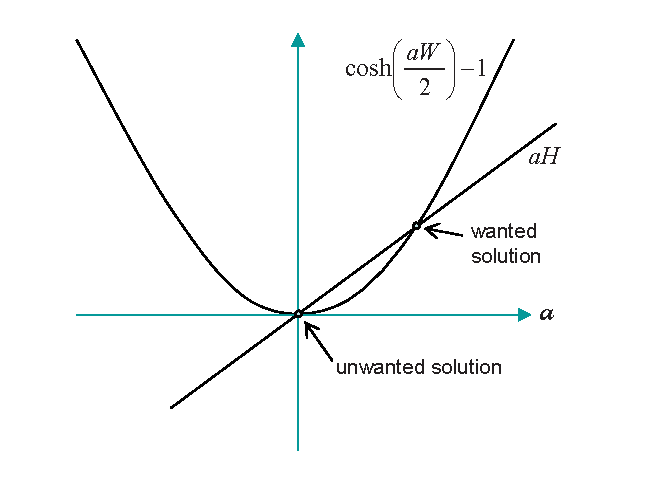
\includegraphics[width=4in]{crosscheck1fig.eps}
\caption{\label{fig:checks}
Visualization of a solution to Eq.~\ref{eq:xcheck1} using a graphical method.
The points marked ``unwanted'' are formally solutions to the equation, but
are not of interest to the experimenter because they are outside of the
physical region of interest in the experiment.}
\end{figure}

\section{Consistency Checks}

To check for consistency in your fit values for $a$ and its error $\Delta a$,
it is useful to estimate $a$ by other methods that require much less data. This
check is also useful to explore how fitting a curve to multiple data points can
afford a more precise measurement of experimental parameters than just solving
using minimal set of measurements. In this experiment, a minimal set of
measurements would entail just measuring two values, which can be chosen to be
either $W$ and $H$, or $W$ and $L$.  Using just these two values and their
errors, it is possible to extract an experimental value for $a$ and its error.
To see how this is done, note that the right suspension point
$(W/2+x_0,H+y_0)$ must lie on the curve given by Eq.~\ref{eq:solfory}, so that
\begin{equation}
aH = \cosh{\frac{aW}{2}}-1
\label{eq:xcheck1}
\end{equation}
Eq.~\ref{eq:xcheck1} is difficult to solve directly, but its graphical solution
is illustrated in Fig.~\ref{fig:checks}. Even though $a = 0$ is formally a
solution, it is not a wanted solution because it implies either that the
tension $T_0$ is infinite, or that $g\lambda = 0$. Use a graphical method
to obtain the intersection indicated in Fig.~\ref{eq:xcheck1}. Excel Solver
would be a good tool to use for this purpose.  The error on
this value is given by
\begin{equation}
\Delta a = \frac{\sqrt{\left(\frac{a}{2}\sinh{\frac{aW}{2}}\right)^2
(\Delta W)^2 + a^2(\Delta H)^2}}
{\left| H-\frac{W}{2}\sinh{\frac{aW}{2}}\right|}
\label{eq:xcheck1err}
\end{equation}
in terms of the measurement uncertainties $\Delta W$ and $\Delta H$.
Compare the value of $a$ obtained using this method with the one obtained
earlier using a fit. Are they consistent? Which method has a smaller
uncertainty?  As a second consistency check, extract $a$ from your
measured values for $W$ and the chain length $L$. The value of $L$
is related to the shape of the chain by computing the integral
\begin{equation}
L=2\int_{x_0}^{x_0+\frac{W}{2}}\sqrt{1+\left(\frac{dy}{dx}\right)^2} dx
\label{eq:lengthint}
\end{equation}
Substitution of the solution Eq.~\ref{eq:solfory} for $y(x)$ leads to the
result
\begin{equation}
aL = 2\sinh{\frac{aW}{2}}
\label{eq:xcheck2}
\end{equation}
which is the analog of Eq.~\ref{eq:xcheck1} using $L$ instead of $H$.
As before, use a graphical method to solve for the wanted solution
of $a$, excluding the unwanted solution $a=0$. The error $\Delta a$
that follows from Eq.~\ref{eq:xcheck2} is
\begin{equation}
\Delta a = \frac{\sqrt{\left(a\cosh{\frac{aW}{2}}\right)^2
(\Delta W)^2 +a^2(\Delta L)^2}}{\left| L-W\cosh{\frac{aW}{2}}\right|}
\label{eq:xcheck2err}
\end{equation}
Verify that the value of $a$ obtained using the $W$,$L$ method agrees
within errors with the value obtained using the $W,H$ method, and also
the one obtained using the curve fitting method. They are in disagreement
if the respective error intervals do not overlap by a factor substantially
greater than 2. If this is the case, work to understand the source of the
discrepancy, or perhaps how you underestimated your errors on one or 
more of the measured parameters.

\section{Finding Roots of Equations Using Graphical Methods}

Excel and most graphing calculators have built-in capability for solving
for the roots of a function within a predetermined interval. Those tools
are suited to the purposes of this course, provided that the student
understands how they work. The experimental physicist must be capable of
finding the roots of equations like Eqs.~\ref{eq:xcheck1} and \ref{eq:xcheck2}
using graphical methods without blindly relying on the output of a tool or
software application.  Internally, these tools rely on iterative algorithms
to home in on a precise value for the root, starting from an initial guess.
Sometimes iterative root finding algorithms are called {\em numerical methods},
but here they are referred to as {\em graphical methods} because they are
only applicable once one knows the global shape of the function in the region
of interest, which implies making (or imagining) a graph of the function.

Root solvers generally start out with a search interval in which a single
root is supposed to lie. The solver then reduces the size of the interval
in successive steps, always making sure that the root lies inside the
remaining interval, until the size of the interval is smaller than the
precision needed for the answer. The following algorithm illustrates this
technique.  It is conceptually very simple. Although it does not converge
as rapidly as other methods like Newton-Raphson, it works in a surprisingly
large number of cases and illustrates how all iterative solvers work.

Suppose the goal is to find the root of the function $f(x)$ between $x_1 = 1$
and $x_2 = 2$. If there is exactly one root in that interval then the
product $f(x_1)f(x_2)$ is less than zero. To reduce the size of the interval,
evaluate $f(x_{av})$ where $x_{av} = (x_1 + x_2)/2$. Evaluate the product
$f(x_av)f(x_1)$.  If it is negative then move the upper bound of the interval
$x_2$ down to $x_{av}$, if it is positive then move the lower bound of the
interval $x_1$ up to $x_{av}$, and if it is zero then return $x_{av}$
as the root. In each step the size of the remaining interval is reduced by
a factor of 2, so that after 30 steps the root is found to a precision of one
part in $10^{9}$.

\begin{acknowledgments}
This document was updated by Prof. Richard Jones, based on an original
write-up by Doug Hamilton (1988), with updates from Prof. Ed Eyler (2004).
\end{acknowledgments}

%% Create the reference section using BibTeX:
%\bibliography{revtex4}

%\begin{thebibliography}{9}
%\bibitem{Cooley65}
%J.W.~Cooley and O.W.~Tukey, {\em An Algorithm for the Machine Calculation of
%Complex Fourier Series}, Math.\ Comput.\ {\bf 19} (1965) pp.\ 297-301.
%\bibitem{Thompson92}
%W.J.~Thompson, {\em Fourier series and the Gibbs Phenomenon}, 
%Am. J. Phys. {\bf 60} (1992) pp.\ 425-429.
%\end{thebibliography}

\end{document}
%%
%% ****** End of file template.aps ******
%
%
